\documentclass[tikz]{standalone}
\usepackage{pgfplots}
\pgfplotsset{compat=1.18}
\definecolor{utnblue}{RGB}{0, 102, 204}

\begin{document}
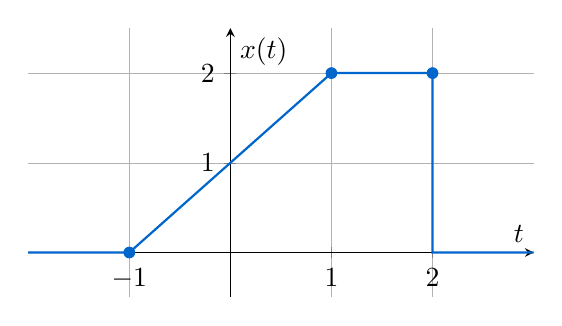
\begin{tikzpicture}
    \begin{axis}[
        width=8cm, height=5cm,
        axis lines=middle,
        xmin=-2, xmax=3, ymin=-0.5, ymax=2.5,
        xlabel={$t$}, ylabel={$x(t)$},
        grid=both,
        grid style={line width=.1pt, draw=gray!40},
        major grid style={line width=.2pt,draw=gray!60},
        xtick={-1,0,1,2},
        ytick={0,1,2},
        every axis plot/.append style={thick},
    ]
    \addplot[utnblue] coordinates {(-2,0) (-1,0) (1,2) (2,2) (2,0) (3,0)};
    % Puntos clave
    \node[circle, fill=utnblue, inner sep=1.5pt] at (-1,0) {};
    \node[circle, fill=utnblue, inner sep=1.5pt] at (1,2) {};
    \node[circle, fill=utnblue, inner sep=1.5pt] at (2,2) {};
    \end{axis}
\end{tikzpicture}
\end{document}
